% !TeX root = ../Baocao.tex
\section{Tính toán, lựa chọn và thiết kế phần cứng UAV}
\subsection{Yêu cầu thiết kế}
Bảng \ref{tab:yeu-cau-phan-cung} tóm tắt các tiêu chí thiết kế
\begin{table}[H]
  \centering
  \caption{Các tiêu chí thiết kế ban đầu của hệ thống}
  \label{tab:yeu-cau-phan-cung}
  \begin{tabularx}{\textwidth}{|>{\raggedright\arraybackslash}p{4.2cm}|>{\raggedright\arraybackslash}X|}
    \hline
    \textbf{Chỉ tiêu} & \textbf{Yêu cầu} \\
    \hline
    Loại UAV & Quadrotor, khung S500, cấu hình chữ X \\
    \hline
    Tải mục tiêu & Tối đa 1~kg; kích thước $15\times10\times10$~cm \\
    \hline
    Máy tính nhúng và camera & Raspberry Pi 5; Raspberry Pi Camera hướng xuống \\
    \hline
    Bộ điều khiển bay & Flight controller chạy PX4 \\
    \hline
    Cơ cấu gắp & Gripper dùng servo; lựa chọn sau khi tính lực và mô-men \\
    \hline
    Thời gian bay yêu cầu & [Bổ sung theo mục tiêu thực nghiệm] \\
    \hline
    Hệ số lực đẩy dự trữ & $k_T=1{,}5$ \\
    \hline
  \end{tabularx}
\end{table}

\subsection{Ước tính khối lượng UAV}

Khối lượng cất cánh toàn bộ của UAV được xác định bằng:
\begin{equation}
  m_{\mathrm{total}}=m_{\mathrm{frame}}+m_{\mathrm{propulsion}}+m_{\mathrm{battery}}+m_{\mathrm{avionics}}+m_{\mathrm{vision}}+m_{\mathrm{gripper}}+m_{\mathrm{payload}},
  \label{eq:tong-khoi-luong-uav}
\end{equation}
trong đó $m_{\mathrm{propulsion}}$ gồm động cơ, ESC và cánh quạt; $m_{\mathrm{avionics}}$ gồm flight controller, Raspberry Pi 5, module nguồn và dây dẫn. 

Khối lượng ước tính này là cơ sở để chọn động cơ và kích thước cánh quạt.

Khối lượng thực sẽ được cân trực tiếp sau khi lắp ráp thay vì chỉ sử dụng giá trị danh định.

\begin{table}[H]
  \centering
  \caption{Bảng cân khối lượng các thành phần UAV}
  \label{tab:ngan-sach-khoi-luong}
  \begin{tabularx}{\textwidth}{|c|>{\raggedright\arraybackslash}X|c|c|}
    \hline
    \textbf{STT} & \textbf{Thành phần} & \textbf{Số lượng} & \textbf{Khối lượng (g)} \\
    \hline
    1 & Khung S500 và càng đáp & 1 & 782 \\
    \hline
    2 & Động cơ, ESC và cánh quạt & 4 bộ & 80x4 \\
    \hline
    3 & Pin và module phân phối nguồn & 1 bộ & 450 \\
    \hline
    4 & Flight controller và cảm biến (GPS, optical, telemetry, receiver)& 1 bộ & 74 \\
    \hline
    5 & Raspberry Pi 5, bộ nguồn và camera & 1 bộ & 147 \\
    \hline
    6 & Gripper, servo và gá lắp & 1 bộ & 145 \\
    \hline
    7 & Kiện hàng & 1 & 1000 \\
    \hline
    \multicolumn{3}{|r|}{\textbf{Tổng khối lượng cất cánh}} & \textbf{2918} \\
    \hline
  \end{tabularx}
\end{table}

\begin{figure}[H]
  \centering
  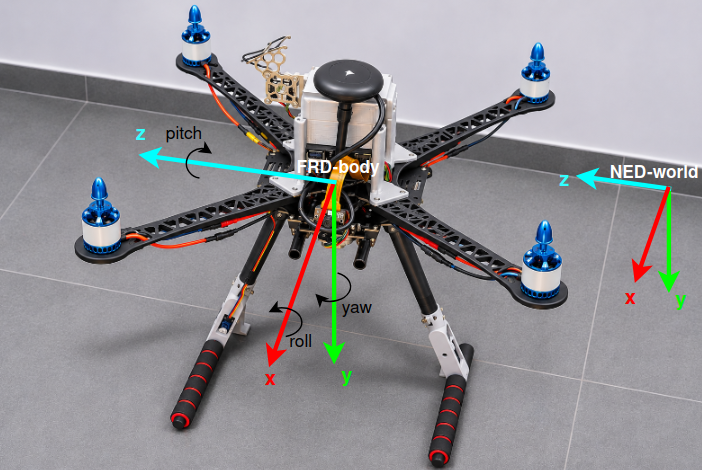
\includegraphics[width=0.6\textwidth]{images/02-uav-model-and-coordinate.png}
  \caption{Cấu tạo phần cứng UAV}
  \label{fig:cau-tao-phan-cung-uav}
\end{figure}

Hình \ref{fig:cau-tao-phan-cung-uav}

\subsection{Tính toán lực đẩy yêu cầu}

Theo Bảng~\ref{tab:ngan-sach-khoi-luong}, khối lượng cất cánh lớn nhất của UAV khi mang tải 1~kg là:
\begin{equation}
  m_{\mathrm{total}}=2918~\mathrm{g}=2{,}918~\mathrm{kg}.
\end{equation}
\indent Ở trạng thái bay treo, tổng lực đẩy của bốn động cơ phải cân bằng trọng lượng UAV:
\begin{equation}
  T_{\mathrm{hover}}=m_{\mathrm{total}}g
  =2{,}918\times9{,}81
  \approx28{,}63~\mathrm{N}.
\end{equation}
\indent Lực đẩy trung bình của mỗi động cơ khi bay treo là:
\begin{equation}
  T_{\mathrm{hover,motor}}
  =\frac{28{,}63}{4}
  \approx7{,}16~\mathrm{N}
\end{equation}
\indent Nếu hệ động lực chỉ tạo lực đẩy xấp xỉ trọng lượng, UAV sẽ phải hoạt động gần mức ga cực đại và không còn đủ dự trữ để tăng độ cao hoặc hiệu chỉnh tư thế. Trong thiết kế này chọn hệ số lực đẩy dự trữ $k_T=1{,}5$, tương ứng tỷ số lực đẩy trên trọng lượng bằng 1,5. Tổng lực đẩy cực đại yêu cầu là:
\begin{equation}
  T_{\mathrm{max,total}}
  \geq k_Tm_{\mathrm{total}}g
  =1{,}5\times28{,}63
  \approx42{,}94~\mathrm{N}
\end{equation}
\indent Do đó, lực đẩy cực đại yêu cầu của mỗi động cơ là:
\begin{equation}
  T_{\mathrm{max,motor}}
  \geq\frac{42{,}94}{4}
  \approx10{,}73~\mathrm{N}
    \approx1094{,}25~\mathrm{gf}.
  \label{eq:luc-day-moi-dong-co}
\end{equation}
\indent Như vậy, mỗi tổ hợp động cơ - 
cánh quạt phải tạo được ít nhất khoảng 
10,73 N tại điện áp pin sử dụng. 
Giá trị này là điều kiện tối thiểu để 
lựa chọn hệ động lực và trong trạng 
thái bay treo đầy tải, mỗi động cơ 
cung cấp khoảng 7,16 N, tương đương khoảng $66{,}7\%$ mức lực đẩy thiết kế cực đại.

\subsection{Lựa chọn động cơ, cánh quạt và ESC}

Động cơ và cánh quạt là hai thành phần quyết định khả năng tạo lực nâng của UAV. Việc lựa chọn cần dựa trên lực đẩy, dòng điện, công suất và khả năng đáp ứng tải trọng của tổ hợp động cơ--cánh quạt.

\noindent\textbf{a) Lựa chọn động cơ}

Từ kết quả tính toán tại mục 2.3, với khối lượng cất cánh lớn nhất 2,918~kg, lực đẩy yêu cầu của mỗi động cơ khi bay treo là 7,16~N, tương đương 729,5~gf. Khi xét hệ số dự trữ lực đẩy $k_T=1{,}5$, mỗi động cơ cần có khả năng tạo lực đẩy cực đại tối thiểu 10,73~N, tương đương khoảng 1.094~gf.

Trên cơ sở đó, đồ án lựa chọn động cơ không chổi than SunnySky X2216-III 950KV. Động cơ sử dụng stator kích thước $22\times16$~mm, có khối lượng danh định 69~g, hỗ trợ nguồn LiPo 3S--4S và công suất cực đại công bố 450~W. Dòng điện cực đại theo thông số kỹ thuật là 32~A trong 30~giây.

Để đánh giá khả năng đáp ứng lực đẩy yêu cầu khi sử dụng pin LiPo 4S, dữ liệu thử nghiệm của nhà cung cấp đối với động cơ SunnySky X2216-III 950KV kết hợp cánh APC 1047 tại điện áp 14,8~V được sử dụng làm cơ sở tham khảo. 
\begin{figure}[H]
  \centering
  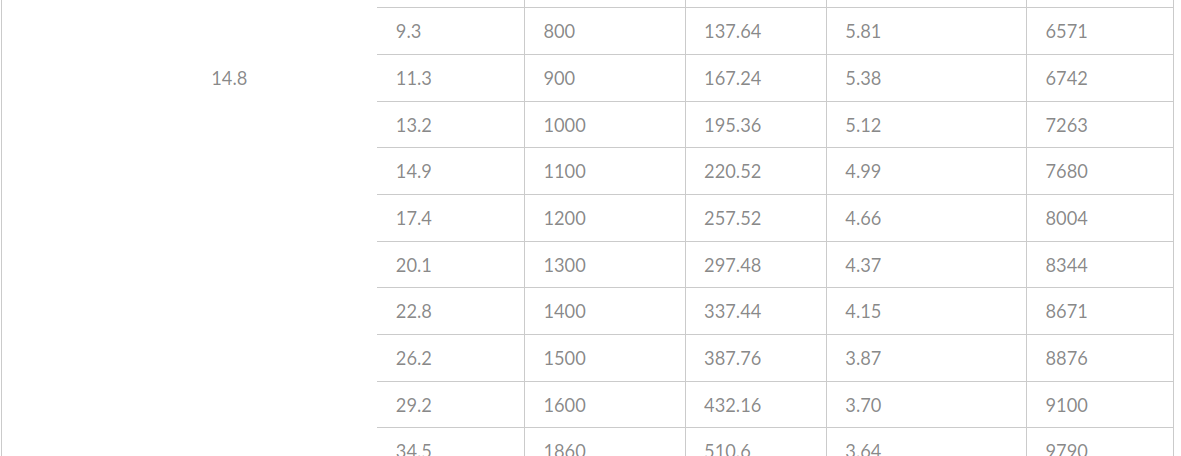
\includegraphics[width=0.8\textwidth]{images/02-specs-sunnysky.png}
  \caption{Dữ liệu thực nghiệm từ nhà cung cấp}
  \label{fig:specs-sunnysky}
\end{figure}
Theo bảng thử nghiệm, tại lực đẩy 800~gf, mỗi động cơ tiêu thụ dòng điện 9,3~A với công suất 137,64~W. Điểm đo này được chọn làm điểm vận hành tham khảo vì lực đẩy 800~gf lớn hơn lực đẩy bay treo yêu cầu 729,5~gf. Khi cả bốn động cơ cùng tạo lực đẩy 800~gf, tổng lực đẩy đạt 3.200~gf, lớn hơn trọng lượng UAV 2.918~gf khoảng 282~gf. Tổng dòng điện và công suất của bốn động cơ tại điểm này lần lượt được ước tính:
\begin{equation}
  I_{\mathrm{total,800}}=4\times9{,}3=37{,}2~\mathrm{A},
\end{equation}
\begin{equation}
  P_{\mathrm{total,800}}=4\times137{,}64=550{,}56~\mathrm{W}.
\end{equation}
\indent Đối với điều kiện lực đẩy lớn, bảng thử nghiệm 4S ghi nhận động cơ đạt 1.100~gf với dòng điện 14,9~A và công suất 220,52~W. Mức lực đẩy này xấp xỉ yêu cầu tối thiểu 1.094~gf đã tính toán tại mục 2.3. Khi biểu diễn cả lực đẩy và trọng lượng theo đơn vị gf, tỷ số lực đẩy trên trọng lượng UAV tại điểm 1.100~gf là:
\begin{equation}
  k_{T,1100}
  =\frac{4T_{1100}}{W_{\mathrm{total}}}
  =\frac{4\times1100}{2918}
  \approx1{,}51.
\end{equation}
Kết quả cho thấy tổ hợp SunnySky X2216-III 950KV và cánh APC 1047 sử dụng pin 4S đáp ứng yêu cầu thiết kế $k_T=1{,}5$ tại điểm thử 1.100~gf.

Bảng thử nghiệm còn ghi nhận lực đẩy lớn nhất 1.860~gf tại 34,5~A và 510,6~W. Khi đó, tỷ số lực đẩy cực đại trên trọng lượng có thể đạt:
\begin{equation}
  k_{T,\max}
  =\frac{4\times1860}{2918}
  \approx2{,}55.
\end{equation}
Tuy nhiên, điểm thử này vượt dòng điện 32~A và công suất 450~W do nhà sản xuất công bố, vì vậy không được xem là chế độ vận hành liên tục an toàn. Đồng thời, tải trọng khuyến nghị cho ứng dụng multirotor thấp hơn mức 729,5~g trên mỗi động cơ của đồ án. Do đó, dòng điện, nhiệt độ và độ ổn định của hệ thống khi bay treo đầy tải với pin 4S cần được kiểm tra bằng thực nghiệm.

\noindent\textbf{b) Lựa chọn cánh quạt}

Bên cạnh dữ liệu của nhà cung cấp, thực nghiệm 
 đối với động cơ SunnySky X2216-III 950KV ghi nhận lực đẩy 1.865~gf với cánh 1045 MR, 
 tương ứng dòng điện 29~A và công suất 455~W. 
 Kết quả này cung cấp bằng chứng thực nghiệm về khả năng tạo lực đẩy lớn của động cơ khi sử dụng cánh 1045.
\begin{figure}[H]
  \centering
  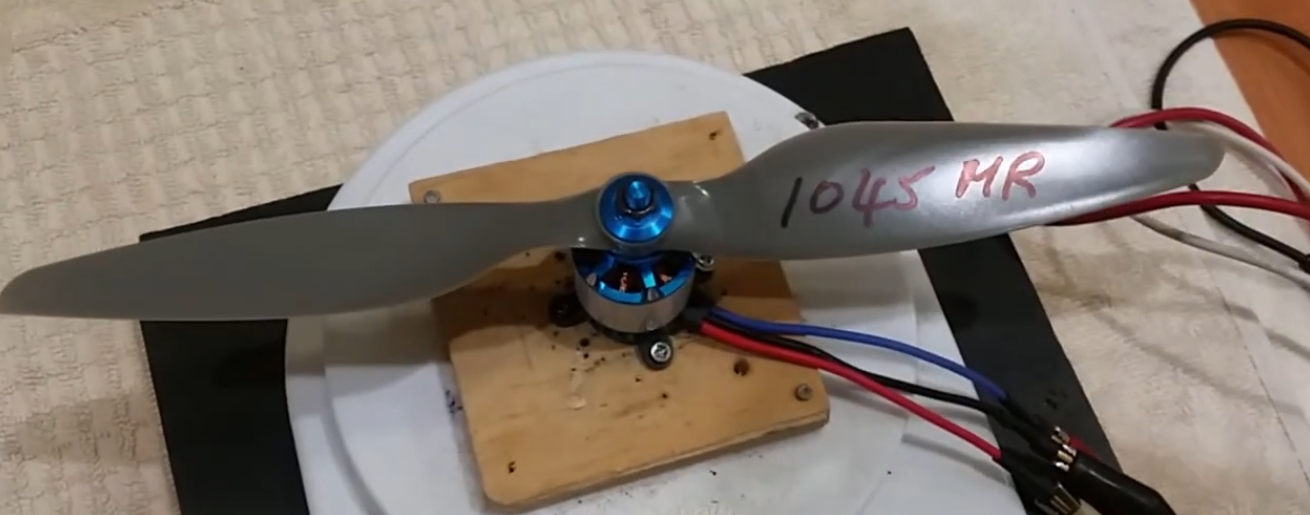
\includegraphics[width=0.6\textwidth]{images/02-ex-sunnysky.png}
  \caption{Thực nghiệm đo lực đẩy của SunnySky X2216-III 950KV với cánh 1045 MR}
  \label{fig:ex-sunnysky}
\end{figure}
\begin{figure}[H]
  \centering
  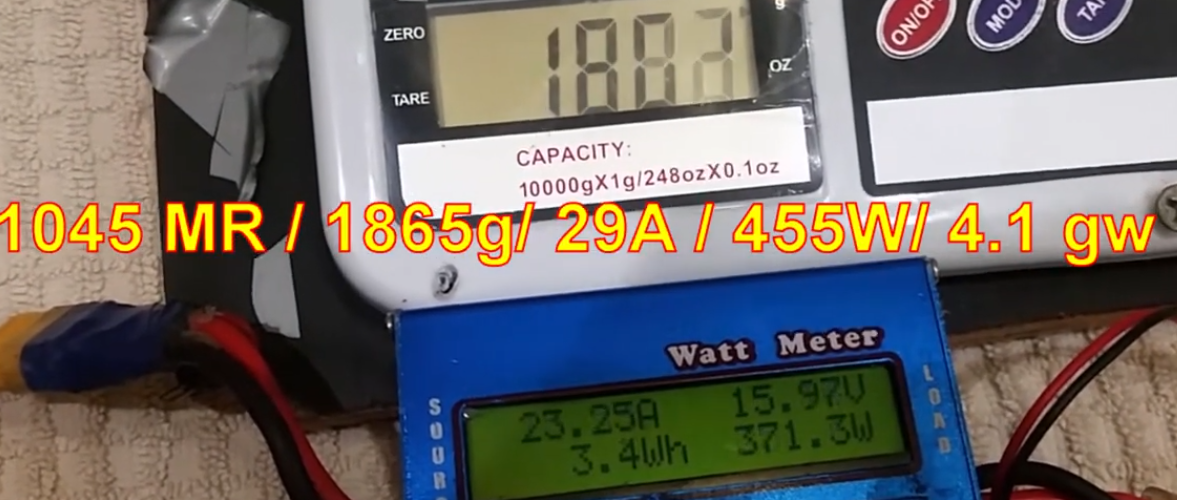
\includegraphics[width=0.6\textwidth]{images/02-ex-data-sunny.png}
  \caption{Thực nghiệm đo lực đẩy của SunnySky X2216-III 950KV với cánh 1045 MR}
  \label{fig:ex-data-sunnysky}
\end{figure}
Từ các dữ liệu khảo sát, tổ hợp động cơ SunnySky X2216-III 950KV và cánh 1045 được lựa chọn làm cấu hình triển khai của đồ án. Lực đẩy, dòng điện và nhiệt độ vận hành cần được kiểm chứng tại điện áp pin sử dụng thực tế nhằm xác nhận khả năng đáp ứng yêu cầu nâng tải 1~kg.

\noindent\textbf{c) Lựa chọn ESC}

Theo thông số kỹ thuật của SunnySky, dòng điện cực đại công bố của động cơ X2216-III 950KV là 32~A trong 30~giây. Với hệ số dự trữ dòng điện $k_I=1{,}2$, dòng định mức tối thiểu của mỗi kênh ESC được xác định:
\begin{equation}
  I_{\mathrm{ESC,rated}}
  \geq k_I\,I_{\mathrm{motor,max}}
  =1{,}2\times32
  =38{,}4~\mathrm{A}.
\end{equation}
Do đó, ESC 4-in-1 có dòng định mức 50~A trên mỗi kênh được lựa chọn nhằm đáp ứng dòng điện của động cơ và tạo khoảng dự trữ trong quá trình tăng lực đẩy khi điều khiển UAV. Bộ ESC phải hỗ trợ điện áp pin sử dụng, đồng thời bảo đảm khả năng tản nhiệt và chịu được tổng dòng điện khi bốn động cơ hoạt động đồng thời.
\subsection{Lựa chọn pin và ước lượng thời gian bay}

Pin được lựa chọn dựa trên điện áp làm việc của hệ động lực, dòng điện yêu cầu, dung lượng và khối lượng. Trong mục 2.4, đặc tính của tổ hợp động cơ SunnySky X2216-III 950KV và cánh APC 1047 được đánh giá tại điện áp 14,8~V. Vì vậy, pin LiPo 4S có điện áp danh định 14,8~V được lựa chọn để bảo đảm điều kiện vận hành phù hợp với dữ liệu tính toán. Điện áp của pin khi sạc đầy có thể đạt 16,8~V, do đó ESC và các bộ chuyển đổi nguồn phải chịu được mức điện áp này.

Tại điểm lực đẩy tham khảo 800~gf trên mỗi động cơ, dòng điện của một động cơ là 9,3~A. Tổng dòng điện của bốn động cơ được xác định:
\begin{equation}
  I_{\mathrm{hover,ref}}=4\times9{,}3=37{,}2~\mathrm{A}.
\end{equation}
Trong trường hợp bốn động cơ đồng thời đạt dòng điện cực đại công bố 32~A, tổng dòng điện cực đại của hệ động lực là:
\begin{equation}
  I_{\mathrm{propulsion,max}}=4\times32=128~\mathrm{A}.
\end{equation}

Từ các yêu cầu trên, đồ án lựa chọn pin LiPo Ovonic 4S1P có dung lượng 5.300~mAh và hệ số xả 75C. Đổi dung lượng pin sang đơn vị ampere-giờ:
\begin{equation}
  C_{\mathrm{Ah}}=5300~\mathrm{mAh}=5{,}3~\mathrm{Ah}.
\end{equation}
Với hệ số xả $C_{\mathrm{rate}}=75C$, dòng xả lý thuyết cực đại của pin là:
\begin{equation}
  I_{\mathrm{battery,max}}
  =C_{\mathrm{rate}}C_{\mathrm{Ah}}
  =75\times5{,}3
  =397{,}5~\mathrm{A}.
\end{equation}
Giá trị này lớn hơn dòng điện cực đại 128~A của bốn động cơ. Hệ số xả tối thiểu cần thiết của pin trong trường hợp cực đại là:
\begin{equation}
  C_{\mathrm{min}}
  =\frac{I_{\mathrm{propulsion,max}}}{C_{\mathrm{Ah}}}
  =\frac{128}{5{,}3}
  \approx24{,}15C.
\end{equation}
Do đó, mức 75C tạo ra khoảng dự trữ dòng điện lớn so với yêu cầu tính toán. Tuy nhiên, giá trị 397,5~A là giá trị lý thuyết theo hệ số C; khả năng chịu dòng thực tế còn phụ thuộc vào đầu nối, dây dẫn, nhiệt độ và giới hạn dòng xả liên tục do nhà sản xuất quy định.

Năng lượng danh định của pin được tính bởi:
\begin{equation}
  E_{\mathrm{battery}}
  =V_{\mathrm{nominal}}C_{\mathrm{Ah}}
  =14{,}8\times5{,}3
  =78{,}44~\mathrm{Wh}.
\end{equation}

Để hạn chế xả sâu, giả sử chỉ sử dụng $\eta_C=80\%$ dung lượng danh định. Lấy dòng điện 37,2~A tại điểm lực đẩy 800~gf làm giá trị tham khảo, thời gian bay lý thuyết được ước lượng:
\begin{equation}
  t_{\mathrm{flight}}
  \approx60\frac{\eta_CC_{\mathrm{Ah}}}{I_{\mathrm{hover,ref}}}
  =60\frac{0{,}8\times5{,}3}{37{,}2}
  \approx6{,}84~\text{phút}.
  \label{eq:thoi-gian-bay}
\end{equation}
Thời gian trên là giá trị ước lượng từ dòng điện của bốn động cơ. Trong thực tế, Raspberry Pi 5, flight controller, camera, servo và tổn hao trên các bộ chuyển đổi nguồn cũng tiêu thụ năng lượng; ngoài ra dòng điện thay đổi theo tải và chế độ bay. Vì vậy, thời gian bay thực tế dự kiến thấp hơn và cần được xác định bằng thử nghiệm. Từ các phân tích về điện áp, khả năng cấp dòng và dung lượng, pin Ovonic 5300~mAh 75C 4S được lựa chọn cho hệ thống.

\subsection{Thiết kế hệ thống cấp và phân phối nguồn}

Hệ thống sử dụng nguồn động lực cho bốn ESC, nguồn ổn định cho flight controller và nguồn phù hợp cho Raspberry Pi 5 cùng servo. Sơ đồ nguồn cần bảo đảm:
\begin{itemize}
  \item dây dẫn, đầu nối và mạch phân phối chịu được dòng cực đại;
  \item bộ DC--DC cấp đủ điện áp và dòng cho Raspberry Pi 5 khi tải tính toán cao;
  \item servo không làm sụt áp hoặc gây khởi động lại Raspberry Pi và flight controller khi hoạt động;
  \item các thiết bị dùng chung mốc điện áp tham chiếu khi truyền tín hiệu;
  \item dây nguồn động lực được bố trí hợp lý với đường tín hiệu và camera để giảm nhiễu.
\end{itemize}

% TODO: Chèn sơ đồ điện, điện áp và dòng định mức của từng nhánh.
\noindent\textit{[Hình cần chèn: Sơ đồ phân phối nguồn từ pin đến ESC, flight controller, Raspberry Pi 5, camera và servo.]}

\subsection{Lựa chọn bộ điều khiển bay và máy tính đồng hành}

Flight controller đảm nhiệm đọc cảm biến quán tính, ước lượng trạng thái và điều khiển ổn định vòng trong. Linh kiện được chọn phải hỗ trợ PX4, có đủ cổng giao tiếp với Raspberry Pi 5 và đủ ngõ ra cho bốn ESC. Sau khi chốt linh kiện, cần ghi rõ mã flight controller, cảm biến, cổng telemetry, giao diện uXRCE--DDS và phương án cấp nguồn.

Raspberry Pi 5 đảm nhiệm thu nhận ảnh, phát hiện ArUco, ước lượng pose, tính lệnh điều khiển cấp cao và điều phối nhiệm vụ. Khi tích hợp cần kiểm tra công suất nguồn, tản nhiệt, bộ nhớ lưu trữ và độ chắc chắn của đầu nối. Giá đỡ nên giảm rung nhưng không được tạo chuyển động tương đối lớn giữa camera và thân UAV.

\begin{table}[H]
  \centering
  \caption{Các thành phần điện tử và chức năng trong hệ thống}
  \label{tab:thanh-phan-dien-tu}
  \begin{tabularx}{\textwidth}{|>{\raggedright\arraybackslash}p{3.7cm}|>{\raggedright\arraybackslash}X|>{\raggedright\arraybackslash}p{3.1cm}|}
    \hline
    \textbf{Thành phần} & \textbf{Chức năng} & \textbf{Giao tiếp/nguồn} \\
    \hline
    Flight controller [mã] & Ổn định bay, đọc cảm biến, điều khiển ESC & [Điền] \\
    \hline
    Raspberry Pi 5 & Xử lý ảnh, điều khiển Offboard, máy trạng thái & [Điền] \\
    \hline
    Raspberry Pi Camera [mã] & Thu ảnh bãi đáp và mã ArUco & CSI; [điền nguồn] \\
    \hline
    Servo [mã] & Đóng/mở cơ cấu gắp & PWM; [điền nguồn] \\
    \hline
  \end{tabularx}
\end{table}

\subsection{Lựa chọn và bố trí camera}

Camera được lắp hướng xuống để quan sát marker trong giai đoạn tiếp cận và hạ cánh. Các tiêu chí lựa chọn gồm độ phân giải, tốc độ khung hình, trường nhìn, độ méo ống kính, giao tiếp với Raspberry Pi 5 và khối lượng. Độ phân giải và tốc độ khung hình phải đủ cho phát hiện marker nhưng không làm thời gian xử lý vượt quá chu kỳ điều khiển.

Camera cần được cố định sao cho trục quang học gần vuông góc với mặt phẳng khung UAV và không bị gripper, kiện hàng hoặc càng đáp che khuất. Sau khi lắp đặt, camera phải được hiệu chuẩn tại đúng độ phân giải sử dụng và xác định phép biến đổi giữa hệ tọa độ camera với hệ tọa độ thân UAV.

% TODO: Chèn ảnh trường nhìn thực tế tại các độ cao thử nghiệm.
\noindent\textit{[Hình cần chèn: Vị trí camera, trục quang học và vùng quan sát marker.]}

\subsection{Tính toán và thiết kế cơ cấu gripper}

Gripper được thiết kế theo kiện hàng $15\times10\times10$~cm, khối lượng tối đa 1~kg. Trước hết cần xác định kiểu giữ vật, hành trình đóng--mở, chiều dài tay kẹp và hệ số ma sát tại bề mặt tiếp xúc.

Đối với cơ cấu kẹp hai phía bằng ma sát, giả sử mỗi má kẹp tác dụng lực pháp tuyến $N$ và hệ số ma sát là $\mu$, điều kiện giữ vật theo phương thẳng đứng là:
\begin{equation}
  2\mu N\geq k_Gm_{\mathrm{payload}}g,
\end{equation}
suy ra lực kẹp tối thiểu trên mỗi má:
\begin{equation}
  N_{\mathrm{min}}=\frac{k_Gm_{\mathrm{payload}}g}{2\mu},
  \label{eq:luc-kep-toi-thieu}
\end{equation}
trong đó $k_G>1$ là hệ số an toàn xét đến rung động và gia tốc khi UAV cất cánh.

Nếu lực từ servo truyền qua tay đòn có chiều dài hiệu dụng $l$, mô-men đầu ra tối thiểu được ước lượng bởi:
\begin{equation}
  \tau_{\mathrm{servo,min}}\geq \frac{N_{\mathrm{req}}l}{\eta_M},
  \label{eq:moment-servo}
\end{equation}
trong đó $\eta_M$ là hiệu suất cơ cấu truyền lực. Nếu dùng bánh răng, thanh truyền hoặc nhiều khớp, cần thay biểu thức trên bằng quan hệ hình học tại vị trí bất lợi nhất của hành trình.

Servo phải đáp ứng mô-men, hành trình, điện áp, tốc độ và khả năng giữ tải. Kết cấu nên có chặn hành trình để tránh kẹt servo, bề mặt tăng ma sát tại má kẹp và phương án xác nhận trạng thái đóng. Khối lượng gripper sau thiết kế phải được cập nhật trở lại bảng ngân sách khối lượng.

\begin{table}[H]
  \centering
  \caption{Các thông số tính toán cơ cấu gripper}
  \label{tab:thong-so-gripper}
  \begin{tabularx}{\textwidth}{|>{\raggedright\arraybackslash}p{4.5cm}|>{\raggedright\arraybackslash}X|}
    \hline
    \textbf{Thông số} & \textbf{Giá trị} \\
    \hline
    Kiện hàng & 1~kg; $15\times10\times10$~cm \\
    \hline
    Hệ số ma sát $\mu$ và hệ số an toàn $k_G$ & [Điền theo vật liệu và yêu cầu] \\
    \hline
    Lực kẹp yêu cầu & [Tính theo phương trình~\eqref{eq:luc-kep-toi-thieu}] \\
    \hline
    Chiều dài tay đòn hiệu dụng & [Điền] \\
    \hline
    Mô-men servo yêu cầu & [Tính theo phương trình~\eqref{eq:moment-servo}] \\
    \hline
    Servo được lựa chọn & [Điền mã, mô-men, tốc độ và điện áp] \\
    \hline
  \end{tabularx}
\end{table}

% TODO: Chèn bản vẽ CAD có kích thước và ảnh gripper mở/đóng.
\noindent\textit{[Hình cần chèn: Cơ cấu gripper, tay đòn, điểm đặt lực và hành trình kẹp.]}

\subsection{Bố trí phần cứng và kiểm tra trọng tâm}

Các linh kiện nặng như pin, Raspberry Pi 5 và gripper cần được bố trí gần tâm hình học của khung. Tọa độ trọng tâm toàn hệ được xác định từ:
\begin{equation}
  \mathbf{r}_{\mathrm{CG}}=\frac{\sum_i m_i\mathbf{r}_i}{\sum_i m_i},
\end{equation}
trong đó $m_i$ và $\mathbf{r}_i$ là khối lượng và vị trí của thành phần thứ $i$. Độ lệch trọng tâm theo phương ngang cần được giảm nhỏ để bốn động cơ có mức tải gần nhau khi bay treo.

Kiện hàng nên được giữ gần trục đứng qua tâm UAV. Nếu tải treo thấp hoặc dao động, mô-men quán tính và nhiễu tư thế tăng; do đó cần rút ngắn khoảng cách treo, tăng độ cứng liên kết và kiểm tra khoảng hở với mặt đất. Camera vẫn phải quan sát được marker trong toàn bộ hành trình hạ cánh và gắp hàng.

% TODO: Chèn bản vẽ lắp tổng thể nhìn từ trên và nhìn bên.
\noindent\textit{[Hình cần chèn: Bố trí phần cứng trên S500 và trọng tâm khi có/không có tải.]}

\subsection{Cấu hình phần cứng và quy trình kiểm tra}

Sau khi lựa chọn linh kiện, cấu hình cuối cùng cần được tổng hợp trong một bảng thông số duy nhất. Trước khi bay, hệ thống được kiểm tra theo từng cấp: kết cấu và chiều quay cánh; nguồn khi chưa lắp cánh; giao tiếp flight controller--Raspberry Pi; camera và servo; động cơ khi cố định khung; bay treo không tải; sau đó tăng tải theo từng mức trước khi thử với 1~kg. Mỗi bước cần ghi lại dòng điện, điện áp pin, nhiệt độ linh kiện và độ ổn định của UAV.

\begin{table}[H]
  \centering
  \caption{Cấu hình phần cứng hoàn chỉnh của UAV}
  \label{tab:cau-hinh-phan-cung-cuoi}
  \begin{tabularx}{\textwidth}{|>{\raggedright\arraybackslash}p{3.8cm}|>{\raggedright\arraybackslash}X|>{\raggedright\arraybackslash}p{3.0cm}|}
    \hline
    \textbf{Cụm} & \textbf{Linh kiện/thông số được chọn} & \textbf{Khối lượng} \\
    \hline
    Khung và càng đáp & S500; [bổ sung chi tiết] & [Điền] \\
    \hline
    Hệ động lực & [Động cơ, cánh quạt, ESC] & [Điền] \\
    \hline
    Nguồn & [Pin, PDB, DC--DC] & [Điền] \\
    \hline
    Điều khiển bay & [Flight controller và cảm biến] & [Điền] \\
    \hline
    Xử lý và thị giác & Raspberry Pi 5; [mã camera] & [Điền] \\
    \hline
    Cơ cấu gắp & [Servo và gripper] & [Điền] \\
    \hline
  \end{tabularx}
\end{table}

\subsection{Tóm tắt chương}

Chương này đã xây dựng quy trình tính toán và lựa chọn phần cứng cho UAV S500 mang tải 1~kg, gồm ngân sách khối lượng, lực đẩy, hệ động lực, pin, phân phối nguồn, flight controller, Raspberry Pi 5, camera và gripper. Các bảng còn để trống sẽ được hoàn thiện bằng dữ liệu linh kiện và kết quả đo thực tế. Đây là cơ sở phần cứng để triển khai các phương pháp thị giác và điều khiển trong Chương 3.
